\section{Реализация системы распределенных вычислений}

В данном разделе описан выбор технологического стека и его роль в реализации
распределённой системы. Подробно обоснован выбор gRPC и Protocol Buffers как
основы сетевого взаимодействия, обеспечивающих строгую типизацию,
производительность и удобство сопровождения кода. Далее рассмотрена реализация
Raft-узла как центрального компонента кластера, включая структуру лога, машину
состояний с механизмом снимков данных, серверный модуль и менеджер заданий.
Приведены ключевые аспекты работы клиентского приложения, включая формат
конфигурационных файлов и двунаправленный потоковый протокол взаимодействия, а
также описана организация вычислительных узлов, их взаимодействие с кластером и
обработка сбоев. В совокупности раздел демонстрирует, каким образом выбранные
технологии и архитектурные решения обеспечивают согласованность состояния,
отказоустойчивость и удобство масштабирования всей системы.

В приложении А приведен протокол всех частей распределенной вычислительной
системы, в приложении Б находится полная UML-диаграмма классов всех частей. В
проекте Abeille \cite{abeille} можно найти полный исходный код.

\subsection{Выбор технологий и инструментов}

Для реализации сетевого взаимодействия в системе был выбран современный
стек \textbf{gRPC + Protocol Buffers}, который обеспечивает эффективную
и строго типизированную коммуникацию между узлами.

gRPC представляет собой высокопроизводительная программная платформа для удалённых
вызовов процедур (Remote Procedure Call, RPC), разработанный компанией Google.
Он использует протокол HTTP/2 на прикладном уровне и TCP на транспортном,
что позволяет реализовать двунаправленные потоки, мультиплексирование
и сжатие заголовков, а также снижает накладные расходы на установку соединений.

Для описания интерфейсов gRPC использует \textbf{.proto}-файлы,
обрабатываемые компилятором Protocol Buffers, который автоматически
генерирует код клиентских и серверных заглушек на выбранных языках.
В рамках данной системы .proto-файлы служат единым источником правды
для определения всех контрактов: как между клиентом и кластером Raft,
так и между внутренними компонентами (сервер, менеджер заданий, рабочий узел).
Это снижает вероятность ошибок согласования интерфейсов,
упрощает сопровождение системы и повышает читаемость кода.

Использование данного стека технологий обеспечивает следующие преимущества:
\begin{itemize}
    \item \textbf{Единая модель данных:} структуры описываются
    один раз в .proto-файлах и автоматически транслируются
    в типобезопасные объекты для всех участвующих компонентов.
    \item \textbf{Удобная сериализация:} поддержка как бинарного,
    так и текстового формата, что упрощает отладку и анализ
    сетевого трафика.
    \item \textbf{Эволюция протокола:} поддержка обратной и
    прямой совместимости при расширении .proto-схем, что позволяет
    постепенно обновлять компоненты системы без остановки кластера.
    \item \textbf{Высокая производительность:} низкие накладные расходы
    на передачу сообщений и эффективная поддержка параллельных
    соединений благодаря HTTP/2.
\end{itemize}

\subsection{Реализация Raft-узла}

Raft-узел является центральным элементом системы: он реализует алгоритм
консенсуса, поддерживает реплицированную машину состояний и предоставляет
интерфейсы для взаимодействия с пользователями и вычислительными узлами.
Реализация узла включает несколько взаимосвязанных компонентов: Raft-лог,
машину состояний с поддержкой снимков данных, серверный модуль, менеджер
заданий и подсистему конфигурации.

\subsubsection{Raft-лог}

Лог Raft представляет собой основной журнал команд, которые подлежат
репликации между всеми узлами кластера. После достижения кворума
запись из лога коммитится и применяется к машине состояний.
В данной реализации поддерживаются две команды:

\begin{itemize}
    \item \texttt{RAFT\_COMMAND\_ADD} — добавление новой задачи в очередь назначенных;
    \item \texttt{RAFT\_COMMAND\_MOVE} — перевод задачи в состояние завершённых.
\end{itemize}

Структура записи лога описана с использованием Protocol Buffers
(см. рис.~\ref{fig:raftlog}). Каждая запись включает тип команды,
номер терма, полезную нагрузку (упакованную в \texttt{TaskWrapper}),
а также дополнительные поля, зависящие от команды
(\texttt{AddRequest} или \texttt{MoveRequest}).
Использование Proto-схемы обеспечивает строгую типизацию,
возможность обратной совместимости при изменении формата и
автоматическую генерацию сериализаторов/десериализаторов.

\begin{figure}[h!]
    \centering
    \includegraphics[width=0.6\linewidth]{inc/raft_log_entry.png}
    \caption{Структура записи Raft-лога, определённая в формате Protocol Buffers.}
    \label{fig:raftlog}
\end{figure}

С точки зрения реализации лог представляет собой потокобезопасную обёртку над
\texttt{std::deque}. Такой выбор объясняется необходимостью обеспечения:

\begin{itemize}
    \item \textbf{Быстрого случайного доступа} по индексу (для алгоритма согласования);
    \item \textbf{Эффективного удаления элементов} как из начала
    (очистка закоммиченных записей после создания снимка данных),
    так и из конца (откат неконсистентных записей при пересинхронизации).
\end{itemize}

Индексация в логе начинается с $1$; нулевой индекс считается невалидным и
используется для упрощения проверок корректности ссылок на записи.

\subsubsection{Машина состояний и механизм снимка данных}

Машина состояний реализует детерминированный автомат, который постепенно
применяет закоммиченные записи лога и формирует текущее состояние кластера. Она
хранит:

\begin{itemize}
    \item список назначенных задач;
    \item список завершённых задач;
    \item текущий номер терма и индекс последней применённой команды.
\end{itemize}

Для предотвращения бесконтрольного роста размера лога реализован механизм
\textbf{снимков данных (snapshotting)}. При достижении порога, заданного
пользователем в конфигурационном файле, машина состояний инициирует создание
снимка данных: сериализует своё текущее состояние и сохраняет его на диск. Данный
процесс выполняется асинхронно, что позволяет продолжать применение новых
команд без блокировки. После успешной записи снимка данных лог очищается от записей,
которые были зафиксированы в сохранённом состоянии, что ограничивает его размер
сверху.

В случае, если лидер не находит в своём логе необходимой записи для
синхронизации с отстающим узлом, он инициирует передачу ему актуального
снимка данных, после чего узел может восстановить своё состояние и продолжить
репликацию с последнего зафиксированного индекса.

\subsection{Серверный модуль}

Серверный модуль инкапсулирует gRPC-сервер, принимающий запросы от:
\begin{itemize}
    \item других узлов (сервис \textbf{RaftService}: \texttt{RequestVote()},
    \texttt{AppendEntries()}, \texttt{InstallSnapshot()});
    \item клиентов (сервис \textbf{UserService});
    \item вычислительных узлов (сервис \textbf{WorkerService}).
\end{itemize}

Сервер маршрутизирует запросы: приём запросов на запись выполняется любым
узлом, но при отсутствии лидерства происходит редирект клиента на лидера.

\subsection{Менеджер заданий}

Task Manager отвечает за подготовку записей для лога Raft при добавлении и
завершении задач, а также за передачу результата пользователю. В реализации
предусмотрены три основных метода:

\begin{itemize}
    \item \texttt{UploadTaskData} — получает данные задачи, выбирает
    идентификатор рабочего узла через \texttt{WorkerServiceImpl::AssignTask()}
    и формирует запись с командой \texttt{RAFT\_COMMAND\_ADD}.
    После успешного выбора рабочего узла запись добавляется в лог Raft
    для репликации и последующего применения к машине состояний.
    \item \texttt{ProcessTask} — передаёт задачу на исполнение выбранному рабочему узлу.
    \item \texttt{UploadTaskResult} — формирует команду
    \texttt{RAFT\_COMMAND\_MOVE}, переводящую задачу из статуса
    \emph{assigned} в \emph{completed}, и добавляет её в лог для
    репликации и коммита.
    \item \texttt{SendTaskResult} — отправляет готовый результат
    обратно в \texttt{UserServiceImpl} для передачи клиенту.
\end{itemize}

Следует отметить, что назначение задачи на рабочего узла выполняется ровно один раз в
момент вызова \texttt{UploadTaskData}. В текущей версии реализации не
предусмотрен механизм автоматического перевыбора рабочего узла или повторной выдачи
задачи при сбое, однако согласованность и идемпотентность обеспечиваются за
счёт самого алгоритма Raft: если запись не была закоммичена до отказа лидера,
она не будет применена к машине состояний, и задача может быть отправлена
повторно клиентом.

\subsubsection{Конфигурация и инициализация узла}

Перед запуском узла пользователь должен предоставить
JSON-конфигурацию (см. рис.~\ref{fig:raftconfig}), в которой указываются:
\begin{itemize}
    \item адреса сервисов (пользовательский, рафт-сервис, сервис рабочего);
    \item список адресов всех узлов кластера (включая данный узел);
    \item параметр \texttt{snapshot\_after} — количество коммитов
    до создания нового снимка данных;
    \item путь к файлу, куда будет записываться снимок данных.
\end{itemize}

\begin{figure}[h!]
    \centering
    \includegraphics[width=0.65\linewidth]{inc/raft_config_example.png}
    \caption{Пример конфигурационного файла Raft-узла.}
    \label{fig:raftconfig}
\end{figure}

В коде конфигурация инкапсулирована в синглтон-объект, который доступен всем
компонентам узла, что упрощает инициализацию и исключает дублирование настроек.
Приложение также поддерживает переопределение некоторых параметров через
аргументы командной строки, что полезно для тестирования и развёртывания в
разных окружениях.

\subsection{Реализация клиентского приложения}

Клиентское приложение предоставляет пользователю консольный интерфейс для
постановки задач на выполнение в кластер и получения результатов. Его
функциональность разбита на несколько подсистем: загрузка конфигураций,
подготовка задания, взаимодействие с кластером, ожидание/получение результата и
сохранение артефактов.

\subsubsection{Конфигурация клиента}

Клиентское приложение конфигурируется с помощью трех файлов. Первый из них
содержит перечень известных адресов узлов Raft. Пример привден на
рис~\ref{fig:client_config}.

\begin{figure}
  \centering
  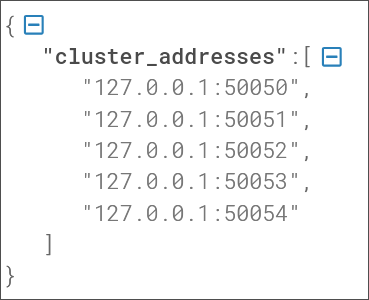
\includegraphics[scale=0.4]{inc/client-config.png}
  \caption{Пример клиентского конфигурационного файла}
  \label{fig:client_config}
\end{figure}

Клиент инициализирует пул соединений к указанным адресам и выбирает рабочую
«точку входа» по порядку (или по доступности). При ошибке соединения
выполняется следующий адрес из списка, что обеспечивает толерантность к отказу
отдельного узла без участия пользователя. Запросы, изменяющие состояние
(постановка задачи), отправляются на любой доступный узел; при необходимости
выполняется прозрачный редирект на лидера.

Второй файл задаёт путь для сохранения результатов и имя динамической
библиотеки задачи (см. рис.~\ref{fig:user_config})

\begin{figure}
  \centering
  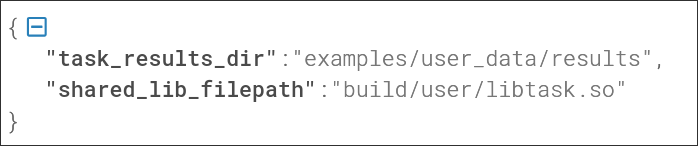
\includegraphics[scale=0.4]{inc/user-config.png}
  \caption{Пример пользовательского конфигурационного файла}
  \label{fig:user_config}
\end{figure}

Третий же файл содержит данные для задания (см. рис.~\ref{fig:user_data}).

\begin{figure}
  \centering
  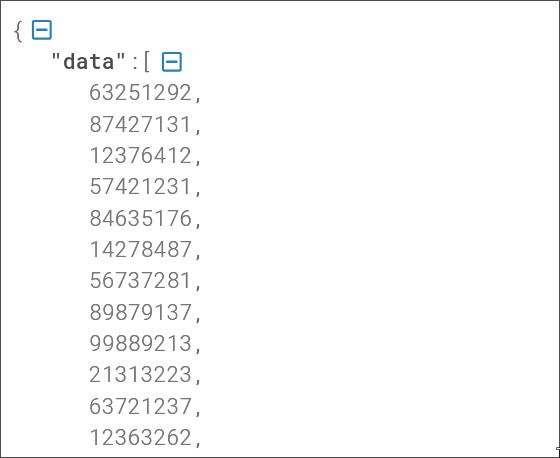
\includegraphics[scale=0.4]{inc/user-data.png}
  \caption{Пример данных для задания}
  \label{fig:user_data}
\end{figure}

\subsubsection{Протокол клиентского приложения}

Взаимодействие клиента с кластером реализовано поверх двунаправленного
потокового вызова \texttt{UserService.Connect}, определённого в gRPC (см. рис
~\ref{fig:user_proto}. Использование потокового RPC позволяет поддерживать
длительное соединение, через которое клиент и сервер обмениваются сообщениями в
обоих направлениях: клиент отправляет последовательность запросов, а сервер —
последовательность ответов, не прерывая сессию. Такой подход позволяет
объединить обнаружение лидера, постановку задачи и получение результата в
единый непрерывный диалог.

\begin{figure}
  \centering
  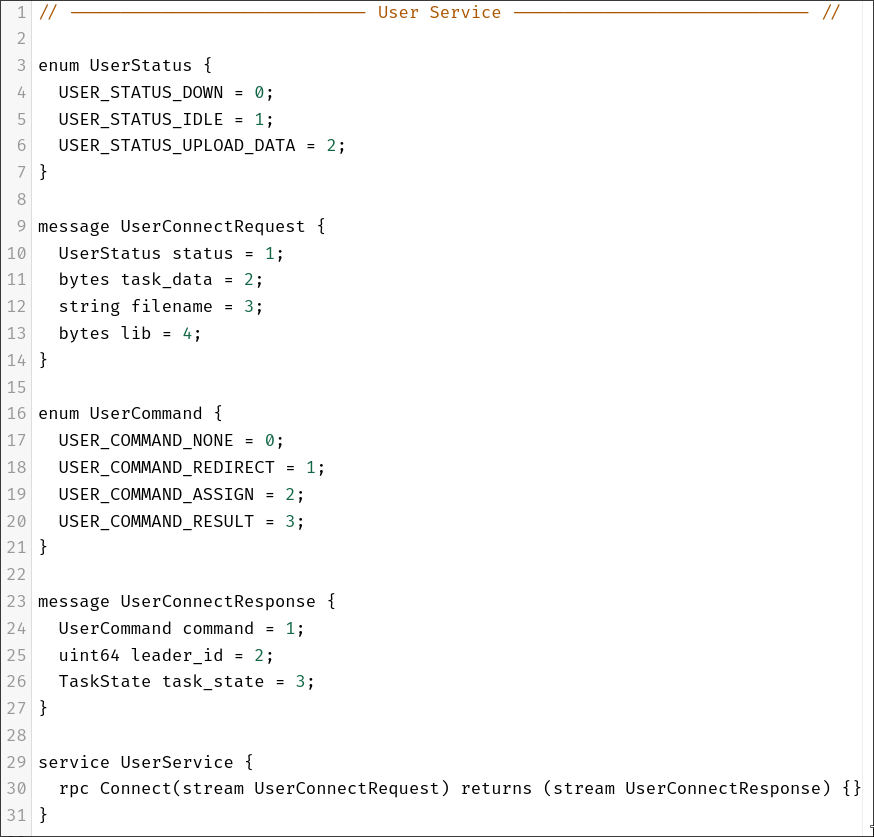
\includegraphics[scale=0.4]{inc/user-proto.png}
  \caption{Протокол общения клиента с кластером Raft}
  \label{fig:user_proto}
\end{figure}

Каждое сообщение клиента содержит поле \texttt{status}, отражающее фазу работы.
На этапе инициализации клиент посылает кадр со статусом \texttt{IDLE},
сигнализируя о готовности к работе. Если узел, на который был направлен запрос,
не является лидером кластера, сервер возвращает ответ с командой \texttt{REDIRECT}
и идентификатором актуального лидера. Получив такую команду, клиент закрывает
поток и устанавливает соединение с указанным узлом, гарантируя, что все
последующие запросы пойдут через единственный согласованный канал.

После установления соединения с лидером клиент переходит к передаче данных
задачи. Для этого используется статус \texttt{UPLOAD\_DATA}, а в сообщении
указываются полезная нагрузка (например, содержимое входного файла),
логическое имя этой нагрузки и идентификатор динамической библиотеки, которая
будет использована при выполнении задачи. Следует подчеркнуть, что по сети
передаётся только имя библиотеки, а не её бинарный образ, поскольку сами
модули заранее развёрнуты на вычислительных узлах. Сервер принимает эти данные,
реплицирует соответствующую команду в Raft-лог, а после достижения кворума
отправляет клиенту ответ с командой \texttt{ASSIGN}, в котором содержится
сгенерированный идентификатор задачи и подтверждение того, что она принята
кластером.

Соединение не разрывается после постановки задачи, а остаётся открытым до
получения финального результата. Когда задача завершается на рабочем узле, её
результат реплицируется через Raft и фиксируется в машине состояний. Лишь
после этого сервер отправляет клиенту команду \texttt{RESULT}, содержащую
окончательный статус выполнения и, при необходимости, сериализованный результат.
Таким образом, клиент всегда получает согласованное состояние, подтверждённое
кворумом узлов.

В совокупности такой протокол обеспечивает упорядоченный и надёжный обмен:
постановка задачи и выдача результата проходят через единую двунаправленную
сессию, которая переносит всю сложность работы с распределённым кластером на
серверную сторону. Клиенту не требуется отслеживать состояние выборов или
дублировать запросы вручную: редиректы, подтверждения и уведомления о результате
получаются автоматически, что делает взаимодействие простым, но при этом
линейризуемым и устойчивым к сбоям.

\subsection{Реализация вычислительного узла}

Вычислительный узел (worker) предназначен для исполнения задач, поступающих из
кластера, и построен вокруг длительного двунаправленного потокового соединения
\texttt{WorkerService.Connect}. При запуске узел считывает локальную
конфигурацию, в которой указывается каталог для размещения динамических
библиотек (\texttt{libs\_dir}) (пример конфигурации приведен на
рис.~\ref{fig:worker_config}). Этот каталог используется как единое хранилище
исполняемых модулей, на которые ссылаются задания. Клиентская часть передаёт
библиотеку в кластер Raft; после репликации и коммита серверная сторона
распределённой системы доставляет содержимое соответствующего артефакта на
вычислительные узлы, где он сохраняется в \texttt{libs\_dir} и становится
доступным среде исполнения.

\begin{figure}
  \centering
  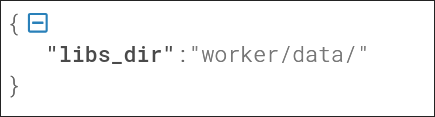
\includegraphics[scale=0.4]{inc/worker-config.png}
  \caption{Пример конфигурационного файла вычислительного узла}
  \label{fig:worker_config}
\end{figure}

Протокол общения вычислительного узла с кластером представлен на
рис.~\ref{fig:worker_proto}.

\begin{figure}
  \centering
  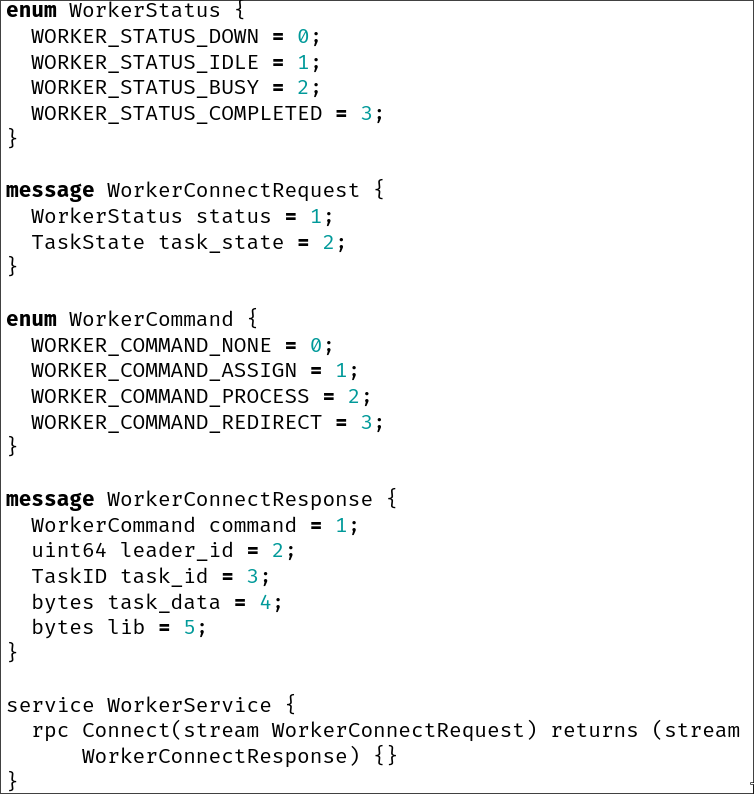
\includegraphics[scale=0.4]{inc/worker-proto.png}
  \caption{Протокол общения вычислительного узла с кластером Raft}
  \label{fig:worker_proto}
\end{figure}

Логика взаимодействия с кластером организована как непрерывная сессия. Сразу
после установления соединения вычислительный узел отправляет кадр с собственным
состоянием \texttt{IDLE}, тем самым сигнализируя о готовности к приёму работы.
Если подключение установлено не с лидером, сервер немедленно возвращает команду
перенаправления с указанием \texttt{leader\_id}; рабочий узел закрывает текущий поток
и повторяет подключение к лидеру, после чего цикл продолжается без участия
оператора. В штатном режиме лидирующий сервер выдаёт команду назначения, в
которой указывает идентификатор задачи и, при необходимости, содержит полезную
нагрузку и бинарные данные библиотеки. В момент получения такого ответа рабочий узел
выполняет атомарную подготовку окружения: проверяет наличие требуемого модуля в
\texttt{libs\_dir}, при отсутствии записывает поступивший образ на диск и
синхронно fsync’ит его, формируя детерминированное имя файла (например, по хешу
содержимого или по имени, пришедшему от сервера), после чего сверяет права
доступа и готовность к загрузке. Этим достигается инвариант, согласно которому
перед запуском пользовательского кода соответствующая библиотека обязательно
присутствует локально и доступна для динамического связывания.

Переход от состояния ожидания к выполнению инициируется командой
\texttt{PROCESS}. Получив её, узел запускает изолированный дочерний процесс
исполняющей среды (в проекте такой процесс может создаваться простым
\texttt{fork()} без сложной контейнеризации), загружает динамическую библиотеку
из \texttt{libs\_dir} и вызывает заранее оговорённый символ интерфейса,
передавая входные данные из \texttt{task\_data}. Основная служба рабочего узла при
этом остаётся в состоянии «занят» и периодически отправляет в поток
\texttt{WorkerConnectRequest} собственный статус и актуальную проекцию
\texttt{TaskState}, обеспечивая наблюдаемость прогресса. В случае штатного
завершения исполняющий процесс формирует результат и отдаёт его основному
процессу узла; далее результат включается в \texttt{TaskState} и возвращается в
кластер тем же потоковым соединением. После этого вычислительный узел переводит
себя в состояние \texttt{COMPLETED}, что служит для серверной стороны сигналом
о готовности зафиксировать завершение в реплицированной машине состояний и
инициировать доставку результата клиенту.

Особое внимание уделено устойчивости к частичным сбоям. Если в ходе выполнения
падает дочерний процесс или попытка динамической загрузки модуля завершается
ошибкой, основная служба не теряет связь с кластером: рабочий узел немедленно
фиксирует ошибочное завершение в \texttt{TaskState} и отправляет его через
активный поток, после чего возвращается в состояние \texttt{IDLE}. Повторы
команд со стороны сервера не приводят к дублированию работы: задача
идентифицируется по \texttt{task\_id}, поэтому рабочий узел либо игнорирует повторные
\texttt{PROCESS} для уже завершённой задачи, либо корректно восстанавливает
исполнение, если сбой произошёл до выдачи финального состояния. Аналогично
сетевые разрывы и смена лидера обрабатываются на транспортном уровне: поток
может быть закрыт с соответствующим статусом gRPC, после чего узел повторяет
подключение с публикацией своего фактического состояния, а серверная сторона,
опираясь на зафиксированные в Raft переходы, восстанавливает согласованную
картину происходящего.

Таким образом, вычислительный узел реализует минимально необходимую
инфраструктуру для безопасного исполнения пользовательского кода: чтение
конфигурации и подготовка каталога библиотек; устойчивое потоковое соединение с
лидером кластера; детерминированная подготовка исполняемого окружения и
загрузка модулей из \texttt{libs\_dir}; изоляция пользовательского исполнения в
отдельном процессе; регулярная публикация статуса и финализация результата
через \texttt{WorkerService.Connect}. Все переходы по состояниям рабочего узла
(\texttt{IDLE} $\rightarrow$ \texttt{BUSY} $\rightarrow$ \texttt{COMPLETED})
отражаются в потоке запросов, а сервер отвечает соответствующими командами
управления и данными (\texttt{ASSIGN}, \texttt{PROCESS}, \texttt{REDIRECT}),
сохраняя линейризуемую семантику наблюдения и единый порядок событий для всех
участников системы.
